\documentclass[a4paper]{article}
\usepackage{answer}
\usepackage{multirow}
\usepackage{subfig}
\usepackage{graphicx}

% Metadata
\date{\today}
\setmodule{ENGG5104 - Image Processing and Computer Vision}
\setterm{Spring 2023}

%-------------------------------%
% Other details
% TODO: Fill these
%-------------------------------%
\title{Assignment 3: Local Feature Matching}
\setmembername{Rongliang Fu}
\setmemberuid{1155186658}

%-------------------------------%
% Add / Delete commands and packages
% TODO: Add / Delete here as you need
%-------------------------------%
\usepackage{amsmath,amssymb,amsthm,bm}

\newcommand{\KL}{\mathrm{KL}}
\newcommand{\R}{\mathbb{R}}
\newcommand{\E}{\mathbb{E}}
\newcommand{\T}{\top}

\newcommand{\expdist}[2]{%
        \normalfont{\textsc{Exp}}(#1, #2)%
    }
\newcommand{\expparam}{\bm \lambda}
\newcommand{\Expparam}{\bm \Lambda}
\newcommand{\natparam}{\bm \eta}
\newcommand{\Natparam}{\bm H}
\newcommand{\sufstat}{\bm u}

% Main document
\begin{document}
% Add header
\header{}

\begin{answer}[Environment]
    \begin{itemize}
        \item Python 3.10.6
        \item Numpy 1.24.2
        \item opencv-python 4.7.0.72
    \end{itemize}
\end{answer}

\begin{answer}[Run]
    cd code \\
    python3 proj2.py
\end{answer}

\textbf{Answer to Result}
\begin{table}[h]
    \begin{tabular}{l|llll|llll}
        \hline
        \multicolumn{1}{c|}{Testcase}           & \multicolumn{4}{c|}{cheat\_interest\_points} & \multicolumn{4}{c}{get\_interest\_points}                                                                                                    \\ \hline
        \multirow{2}{*}{num\_pts\_to\_evaluate} & \multicolumn{2}{c}{no limit}                 & \multicolumn{2}{c|}{100}                  & \multicolumn{2}{c}{no limit} & \multicolumn{2}{c}{100}                                           \\ \cline{2-9}
                                                & accuracy                                     & runtime                                   & accuracy                     & runtime                 & accuracy & runtime & accuracy & runtime \\ \hline
        Notre Dame                              & 63.76\%                                      & 0.72 s                                    & 79.00\%                      & 0.61 s                  & 45.30\%  & 19.76 s & 100\%    & 20.96 s \\
        Mount Rushmore                          & 40.48\%                                      & 0.54 s                                    & 46.00\%                      & 0.57 s                  & 4.93\%   & 22.35 s & 63.00\%  & 22.37 s \\
        Episcopal Gaudi                         & 13.70\%                                      & 0.61 s                                    & 18.00\%                      & 0.61 s                  & 2.87\%   & 19.99 s & 16.00\%  & 19.72 s \\ \hline
    \end{tabular}
\end{table}

\textbf{Answer to visualization}
\begin{figure}[h]
    \centering
    \subfloat[My result of Notre Dame]{\includegraphics[width=1\textwidth]{result/Notre_100_vis_dots_result.png}}
\end{figure}
\begin{figure}[h]
    \centering
    \ContinuedFloat
    \subfloat[My result of Mount Rushmore]{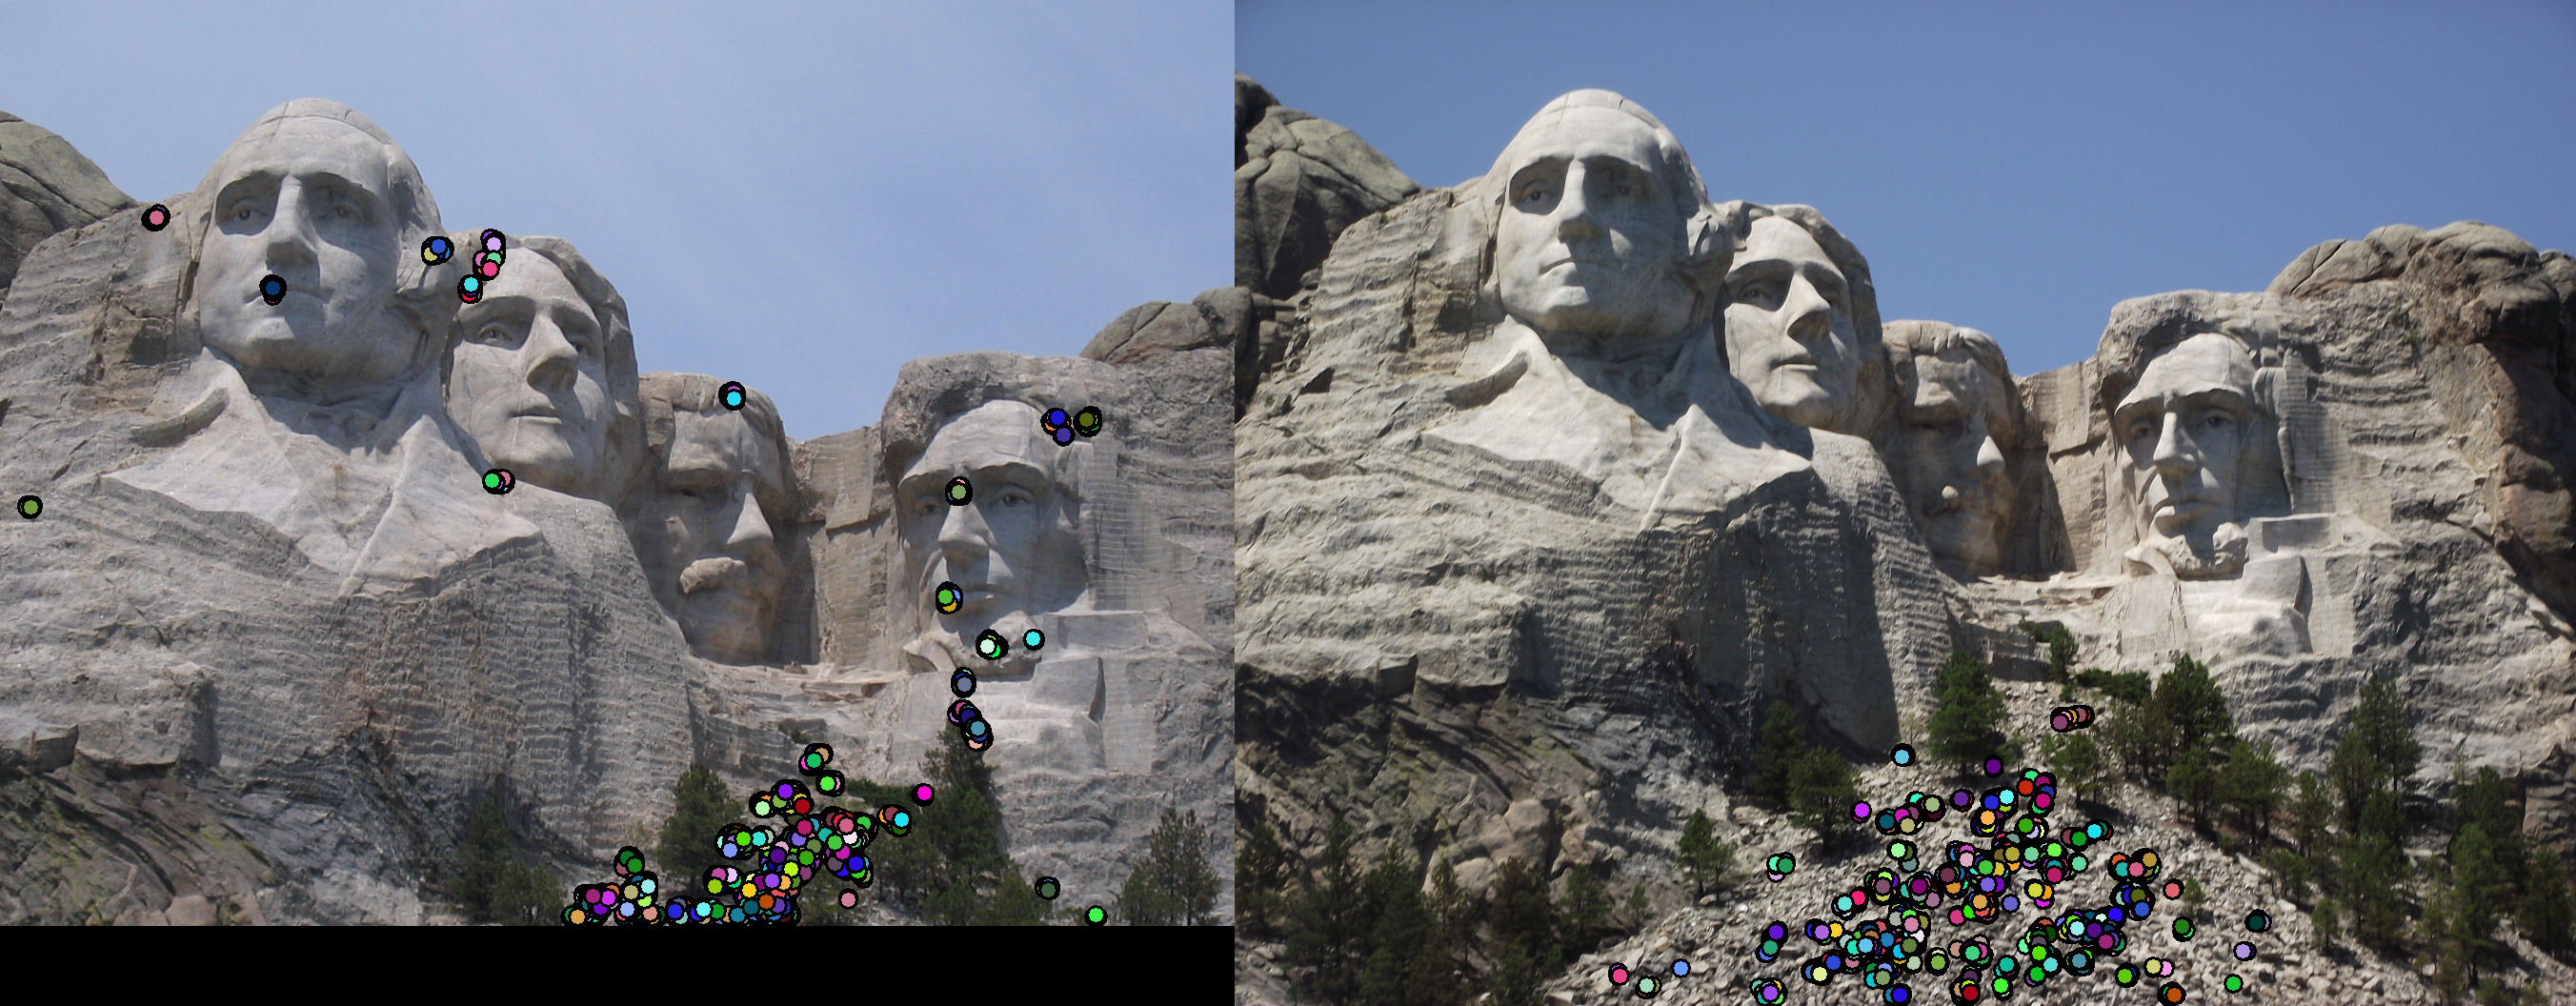
\includegraphics[width=1\textwidth]{result/Mount_100_vis_dots_result.png}} \\
    \subfloat[My result of Episcopal Gaudi]{\includegraphics[width=1\textwidth]{result/Episcopal_100_vis_dots_result.png}} \\
    \subfloat[My result of my office]{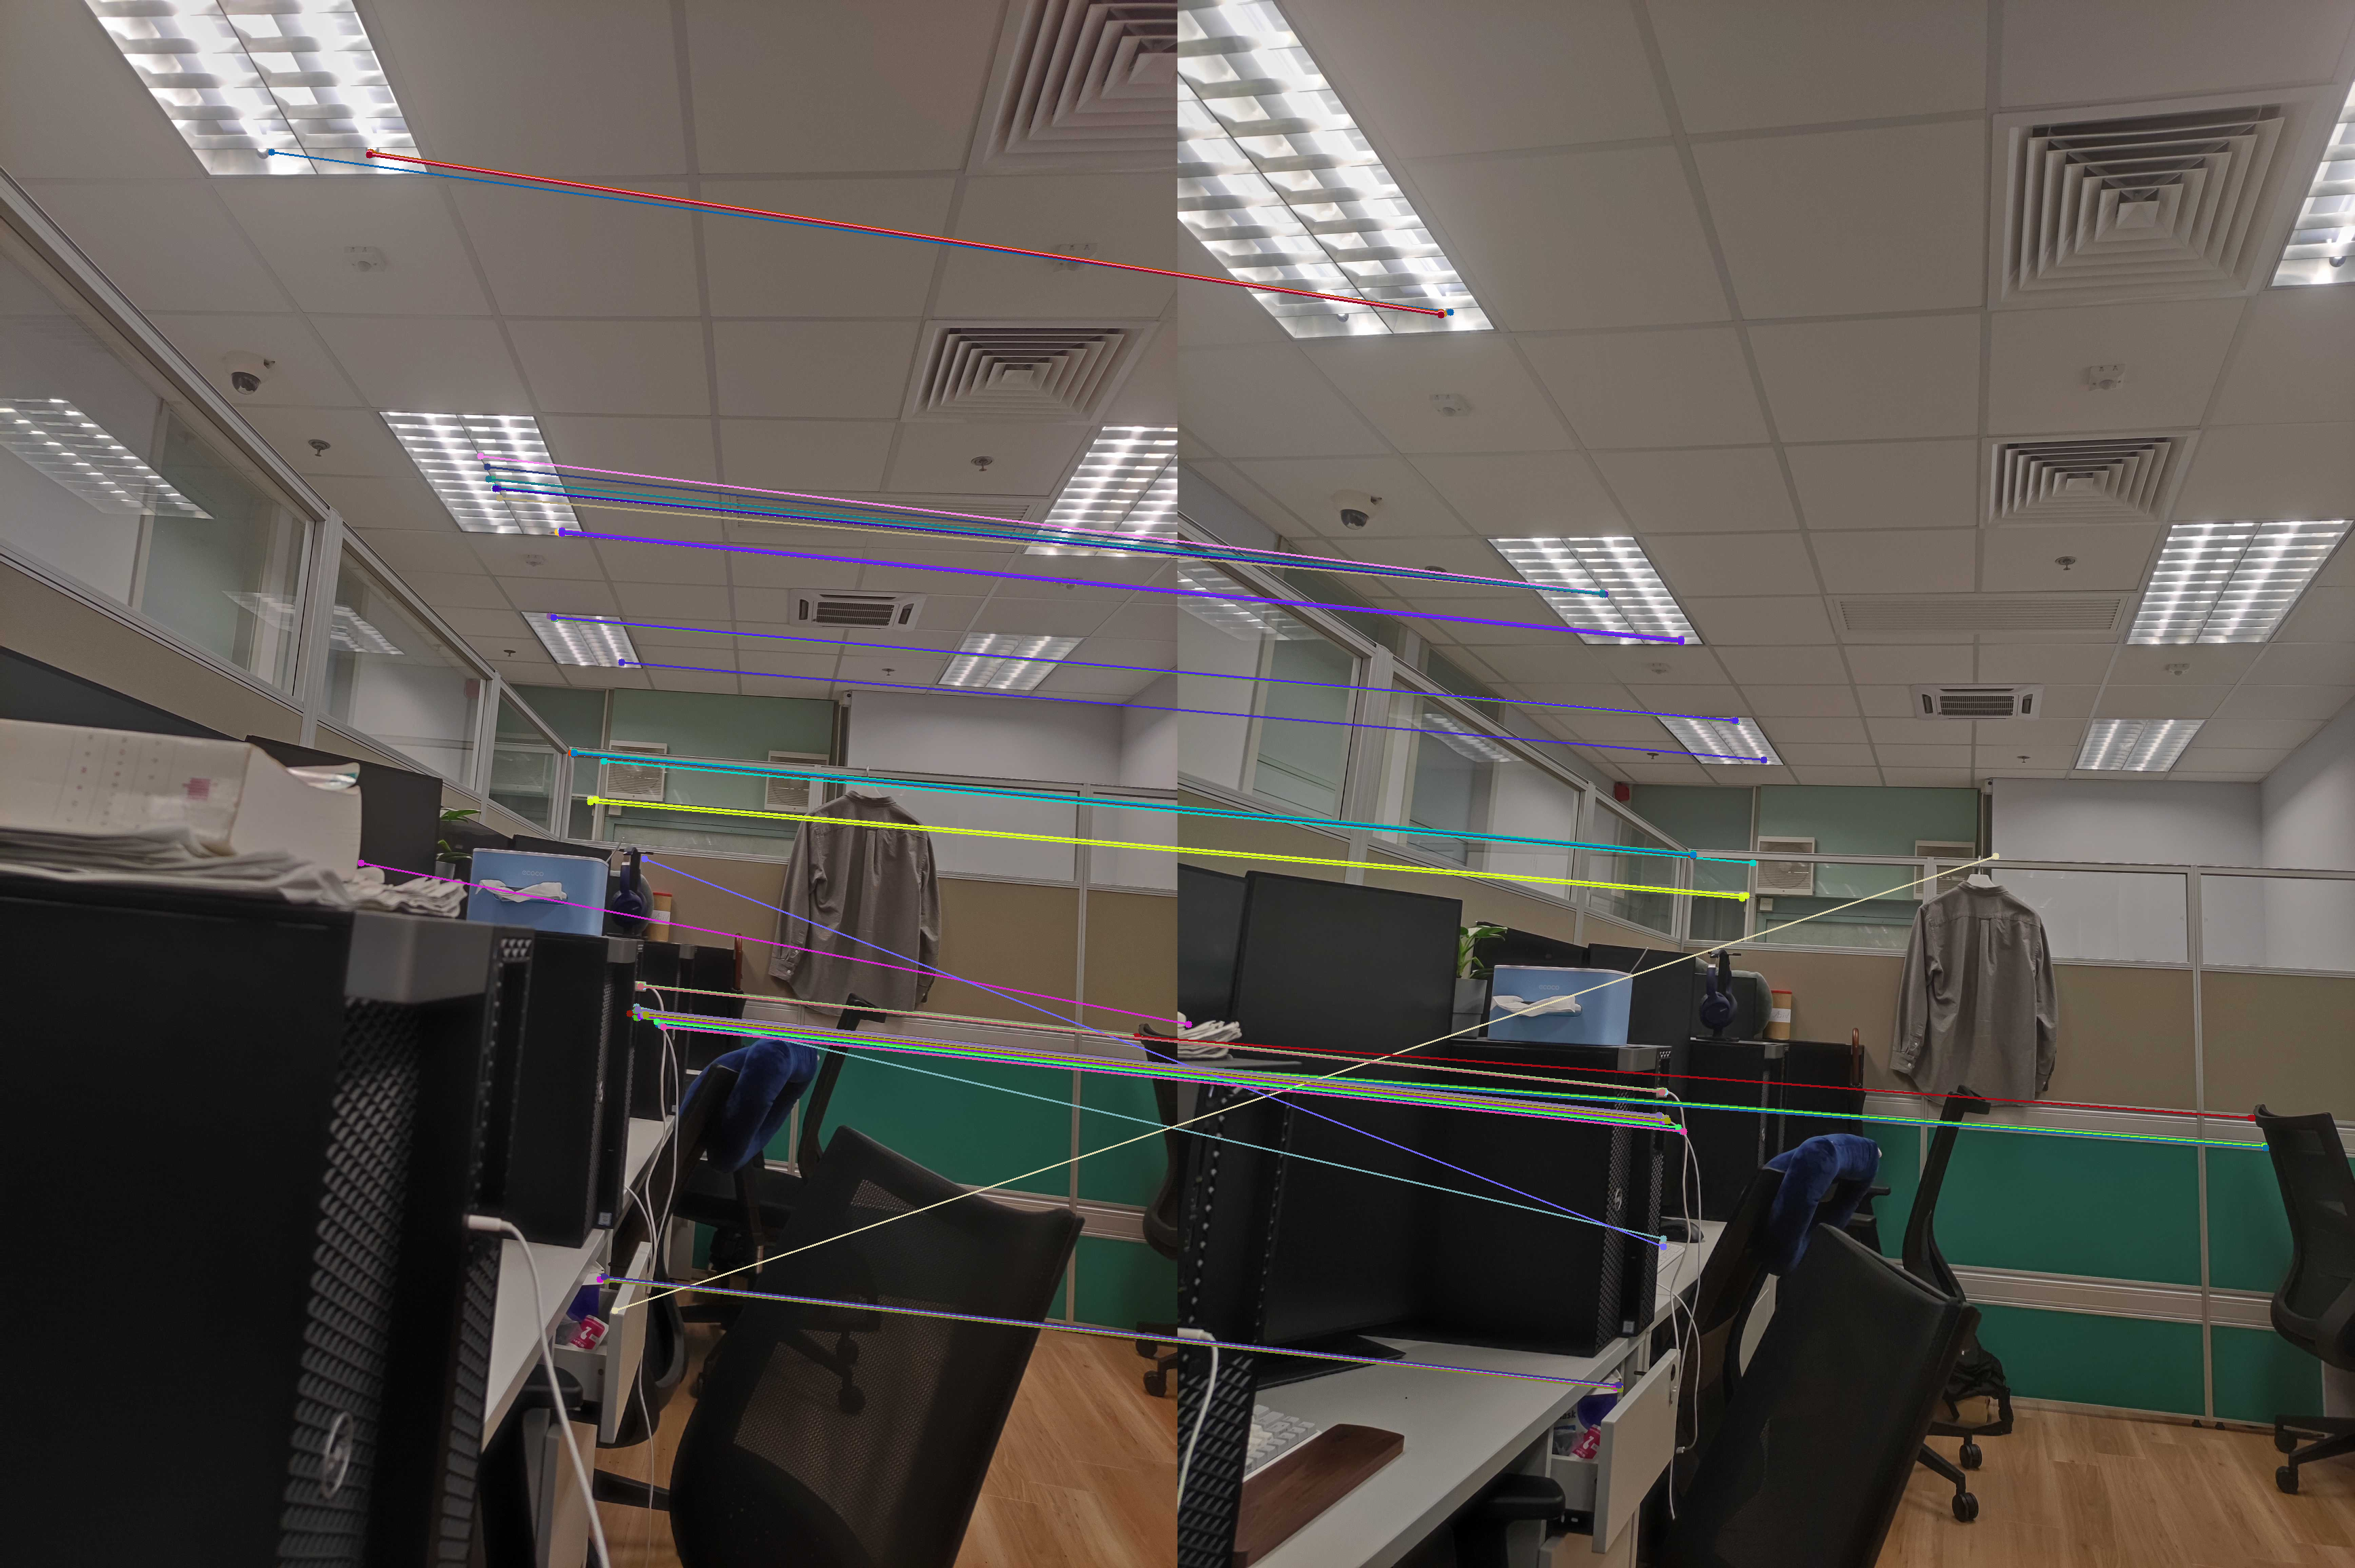
\includegraphics[width=1\textwidth]{result/vis_arrows_result.png}}\vspace{3pt}
\end{figure}


\end{document}
